\documentclass[12pt,letterpaper,titlepage,en-US]{article}

\usepackage{basicstyle}
\usepackage{report}
\usepackage{knit}
\usepackage{amsmath}
\usepackage{xcolor}
\usepackage{listings}
\usepackage{fancyvrb}
\usepackage{graphicx}
\definecolor{lbcolor}{rgb}{0.969, 0.969, 0.969} 

 \lstset{ 
    language=R, % choose the language of the code
    basicstyle=\fontfamily{pcr}\selectfont\footnotesize\color{black},
    keywordstyle=\color{black}, % style for keywords
    numbers=none, % where to put the line-numbers
    numberstyle=\tiny, % the size of the fonts that are used for the line-numbers     
    backgroundcolor=\color{lbcolor},
    showspaces=false, % show spaces adding particular underscores
    showstringspaces=false, % underline spaces within strings
    showtabs=false, % show tabs within strings adding particular underscores
    frame=single, % adds a frame around the code
    tabsize=2, % sets default tabsize to 2 spaces
    rulesepcolor=\color{gray},
    rulecolor=\color{black},
    captionpos=b, % sets the caption-position to bottom
    breaklines=true, % sets automatic line breaking
    breakatwhitespace=false, 
}


\newcommand{\hmwkTitle}{Mini Project \#4}
\DTMsavetimestamp{DueDate}{2019-04-11T10:00:00-06:00}
\newcommand{\hmwkClass}{CS 6313.001}
\newcommand{\hmwkClassName}{Statistical Methods for Data Science}
\newcommand{\hmwkClassInstructor}{Instructor: Prof. Min Chen}
\newcommand{\hmwkAuthorName}{Shyam Patharla}
\newcommand{\hmwkAuthorNetID}{sxp178231}

\newcommand{\hmwkAuthorOneName}{Lizhong Zhang (lxz160730) : P1(ae), P2(bcde)}
\newcommand{\hmwkAuthorTwoName}{Hanlin He (hxh160630) : P1(bcd), P2(af)}



%
% Title Page
%

\title{
    \vspace{1in}
    \textmd{\textbf{\hmwkClassName \\\hmwkClass:\ \hmwkTitle }}\\
     \normalsize\vspace{0.1in}\small{Due\ on\ \DTMusedate{DueDate}\ at \DTMusetime{DueDate} }\\
    \vspace{0.1in}\large{\textit{\hmwkClassInstructor}}\\
    \vspace{0.5in}
\includegraphics[height=2.4em]{UTD_logo_BW}\\
    \vspace{2in}
}

\author{\textbf{\hmwkAuthorName\ \footnotesize{(\hmwkAuthorNetID)}} \\ }
\date{}
\makeindex

\begin{document}
\maketitle

\pagenumbering{Roman}

\tableofcontents

\pagebreak
\pagenumbering{arabic}


\section{Answers}

\subsection{}

\subsubsection{Scatterplot of GPA against ACT}
We get the following scatterplot of gpa scores vs act scores:
\begin{knitrout}
\definecolor{shadecolor}{rgb}{0.969, 0.969, 0.969}\color{fgcolor}
\begin{kframe}
\begin{verbatim}
> plot( gpa, act.scores, xlab="gpa", ylab="ACT score",
main = "Scatterplot: GPA vs ACT scores")
> abline( lm (act.scores~gpa))
\end{verbatim}
\end{kframe}
\end{knitrout}
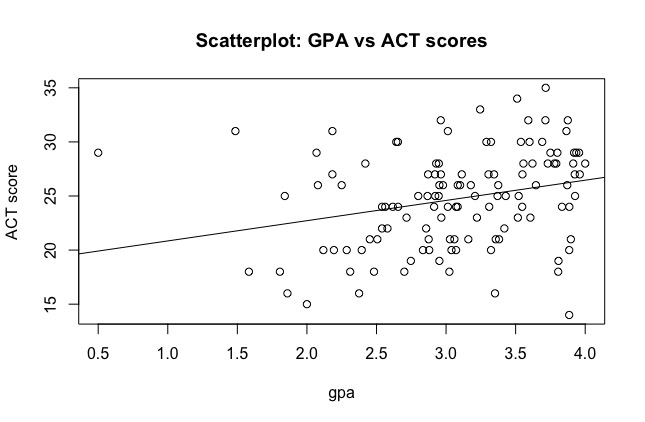
\includegraphics[scale=0.6]{scatterplot.jpeg}\\


Conclusions:
\begin{enumerate}
\item The relationship between gpa scores and act scores for the given sample is \textbf{not} a very linear relationship.
\item For students having a high gpa, there are almost equal number of students having a low act score and a high act score
and hence a high gpa \textbf{does not} necessarily correspond to a high act score.
\item For students having a low gpa, there are almost equal number of students having a low act score and a high act score and hence a low gpa \textbf{does not} necessarily correspond to a low act score.
\end{enumerate}

\subsubsection{Point estimate of population correlation}
We need to estimate the population correlation between X and Y, where X is the GPA distribution and Y is the ACT scores distribution.

\begin{equation}
\theta = \rho (X,Y)
\end{equation}


We compute the point estimate of $\theta$ using the \textbf{cor()} function:
\begin{knitrout}
\definecolor{shadecolor}{rgb}{0.969, 0.969, 0.969}\color{fgcolor}
\begin{kframe}
\begin{verbatim}
> cor(gpa,act.scores)
# [1] 0.2694818 
\end{verbatim}
\end{kframe}
\end{knitrout}

So, we have $\hat{\theta}$ = 0.26984818.



\subsubsection{Bootstrap estimates of bias and standard error of the point estimate}
We get the bootstrap statistics using:
\begin{knitrout}
\definecolor{shadecolor}{rgb}{0.969, 0.969, 0.969}\color{fgcolor}
\begin{kframe}
\begin{verbatim}
> corr.npar.boot <- boot(data,corr.npar,sim="ordinary",R=1000)
# ORDINARY NONPARAMETRIC BOOTSTRAP
# Call:
#  boot(data = data, statistic = corr.npar, R = 1000, sim = "ordinary")
# Bootstrap Statistics :
#  original      bias    std. error
# t1* 0.2694818 0.001159284   0.1071447
\end{verbatim}
\end{kframe}
\end{knitrout}
where \textbf{corr.npar} is a function for bootstrap sampling.\\

Bootstrap estimate for E($\hat{\theta}$) = original + bias = 0.2706411,
$Std(\hat{\theta}) = 0.1071447
$


\subsubsection{95 per cent confidence interval computed using percentile bootstrap}

\begin{knitrout}
\definecolor{shadecolor}{rgb}{0.969, 0.969, 0.969}\color{fgcolor}
\begin{kframe}
\begin{verbatim}
> boot.ci(corr.npar.boot,conf=0.95)
# BOOTSTRAP CONFIDENCE INTERVAL CALCULATIONS
# Based on 1000 bootstrap replicates
# CALL : 
# boot.ci(boot.out = corr.npar.boot, conf = 0.95)
# Intervals : 
# Level      Normal              Basic         
# 95%   ( 0.0583,  0.4783 )   ( 0.0546,  0.4808 )  
# Level     Percentile            BCa          
# 95%   ( 0.0582,  0.4844 )   ( 0.0393,  0.4723 ) 
\end{verbatim}
\end{kframe}
\end{knitrout}
The 95\% CI computed using percentile bootstrap is \textbf{[0.0582,0.4844]}.\\

Conclusions:
\begin{enumerate}
\item The mean of the bootstrap distribution for the population correlation  estimator is very close to the sample correlation.

\begin{knitrout}
\definecolor{shadecolor}{rgb}{0.969, 0.969, 0.969}\color{fgcolor}
\begin{kframe}
\begin{verbatim}
> mean(corr.npar.boot$t)-corr.npar.boot$t0
# [1] -1.650308e-05

> cor(gpa,act.scores)
# [1] 0.2694818 

> corr.npar.boot$t0
# [1] 0.2694818
\end{verbatim}
\end{kframe}
\end{knitrout}


\item The standard deviation of the bootstrap distribution is quite low.
\begin{knitrout}
\definecolor{shadecolor}{rgb}{0.969, 0.969, 0.969}\color{fgcolor}
\begin{kframe}
\begin{verbatim}
> sd(corr.npar.boot$t)
# [1] 0.104966
\end{verbatim}
\end{kframe}
\end{knitrout}

\item The bootstrap estimate of the population correlation is positive ($\theta=0.2706411$), which \textbf{agrees} with our scatterplot, which shows a \textbf{positive slope line} to be fitting the data.

\item The estimated value of the population correlation is \textbf{not very high}, and this is evident from the scatterplot that the data does not fit the line well.
\end{enumerate}

The histogram of the bootstrap distribution is obtained\\
\includegraphics[scale=0.6]{histBoot.jpeg}\\


\subsection{}
\subsubsection{Exploratory analysis of the local and remote voltages distributions}
We make a boxplot and histograms for both the distributions:\\
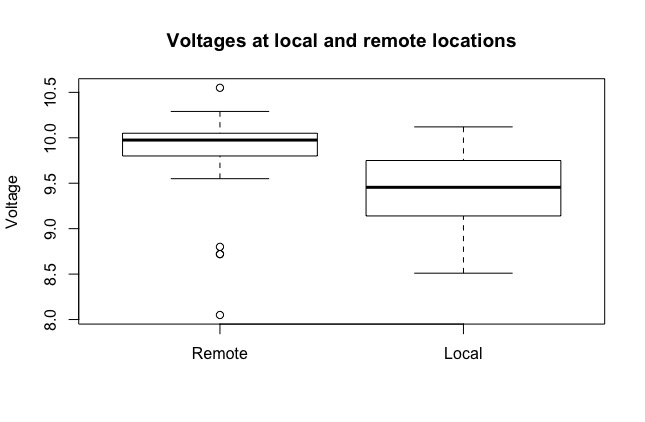
\includegraphics[scale=0.6]{boxplot2A.jpeg}\\
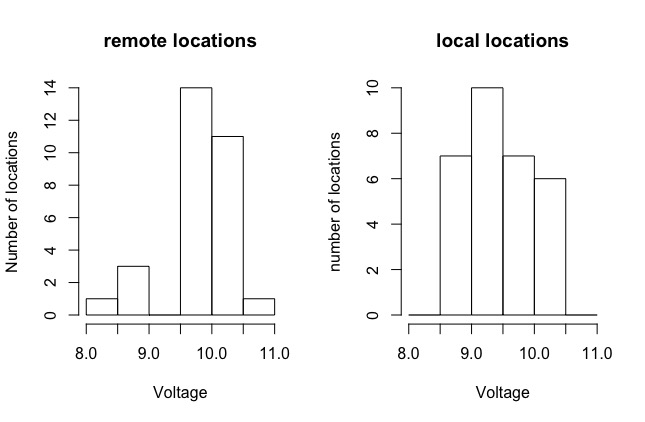
\includegraphics[scale=0.6]{hist2A.jpeg}\\

Inferences:
\begin{enumerate}
\item The distributions are quite\textbf{ different}. 
\item The remote voltages distribution has a \textbf{higher} median and  a \textbf{narrower} inter-quartile range than the lower voltages distribution.
\item The values in the remote voltages distribution are in general \textbf{higher} than the values in the local voltages distribution.
\item The remote voltages distribution has a slightly \textbf{higher mean}.
\begin{knitrout}
\definecolor{shadecolor}{rgb}{0.969, 0.969, 0.969}\color{fgcolor}
\begin{kframe}
\begin{verbatim}
> mean(voltage.remote)
# [1] 9.803667
> mean(voltage.local)
# [1] 9.422333
\end{verbatim}
\end{kframe}
\end{knitrout}
\item The remote voltages distribution has \textbf{outliers} on both extremes, in contrast to the local voltages which do not have outliers.
\item The histograms show similar arguments.



\item We can conclude that the remote voltages and local voltages do not have similar distributions.
\end{enumerate}

\subsubsection{Can the manufacturing process be established locally?}
We must estimate the difference in means of the two populations. Hence;
\begin{equation}
\theta = \mu_{X} - \mu_{Y}
\end{equation}
where $\mu_{X}$ is the mean of the remote voltages and $\mu_{Y}$ is the mean of the local voltages. We first get an estimator for $\theta$:
\begin{knitrout}
\definecolor{shadecolor}{rgb}{0.969, 0.969, 0.969}\color{fgcolor}
\begin{kframe}
\begin{verbatim}
> mean.diff.estimator <- x.mean - y.mean
> mean.diff.estimator
# [1] 0.3813333
\end{verbatim}
\end{kframe}
\end{knitrout}

We assume the 2 populations have \textbf{equal variances} since the same devices are used to measure voltages at both locations.
\begin{equation}
\sigma_{1}^{2} = \sigma^{2}_{2}= \sigma^{2}
\end{equation}

We get a pooled sample variance for both the distributions:
\begin{knitrout}
\definecolor{shadecolor}{rgb}{0.969, 0.969, 0.969}\color{fgcolor}
\begin{kframe}
\begin{verbatim}
> pooled.var <- ( (n-1 )* x.var + (m-1) * y.var) / (n+m-2)
\end{verbatim}
\end{kframe}
\end{knitrout}

Finally, we get the confidence interval for $\theta$
\begin{knitrout}
\definecolor{shadecolor}{rgb}{0.969, 0.969, 0.969}\color{fgcolor}
\begin{kframe}
\begin{verbatim}
> mean.diff.ci <-  mean.diff.estimator + c(-1,1) *
 qt(1-(1-0.95), n+m-2) * sqrt(pooled.var/m + pooled.var/n)
> print(mean.diff.ci)
# [1] 0.1173110 0.6453556
\end{verbatim}
\end{kframe}
\end{knitrout}

The confidence interval suggests that the difference in means is \textbf{positive} and hence, the manufacturing process \textbf{cannot} be replicated locally.


\subsubsection{Compare conclusions drawn in (b) to the results of exploratory analysis in (a)}
The conclusions drawn in both (a) and (b) are similar and indicate that the process \textbf{cannot} be replicated locally.

\subsection{}
We first make boxplots and histograms for the theoretical and experimental vapor pressure distributions.\\
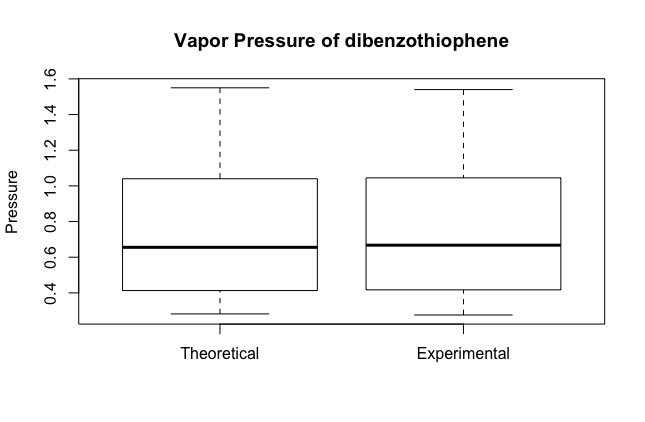
\includegraphics[scale=0.6]{boxplot3.jpeg}\\




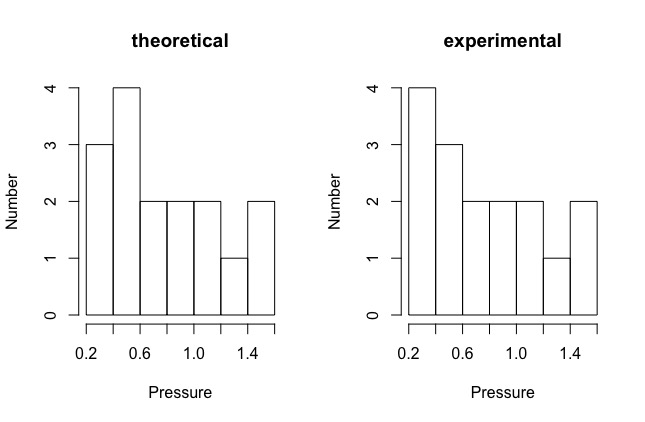
\includegraphics[scale=0.6]{hist3.jpeg}\\

Exploratory analysis:
\begin{enumerate}
\item The boxplots show that the two distributions are quite \textbf{similar}.
\item They have similar medians, interquartile ranges and are almost identical.
\item The histograms are identical except for the case of the first two buckets.
\end{enumerate}
We must estimate the difference in means of the two populations. Hence;
\begin{equation}
\theta = \mu_{X} - \mu_{Y}
\end{equation}
where $\mu_{X}$ is the mean of the theoretical values and $\mu_{Y}$ is the mean of the experimental values. We first get an estimator for $\theta$:
\begin{knitrout}
\definecolor{shadecolor}{rgb}{0.969, 0.969, 0.969}\color{fgcolor}
\begin{kframe}
\begin{verbatim}
> mean.diff.estimator <- x.mean - y.mean
> mean.diff.estimator
# [1] 0.0006875
\end{verbatim}
\end{kframe}
\end{knitrout}


We \textbf{assume} the 2 populations have equal variances since the sample variances are very close to each other.
\begin{equation}
\sigma_{1}^{2} = \sigma^{2}_{2}= \sigma^{2}
\end{equation}
\begin{knitrout}
\definecolor{shadecolor}{rgb}{0.969, 0.969, 0.969}\color{fgcolor}
\begin{kframe}
\begin{verbatim}
> x.var
# [1] 0.1643551
> y.var
# [1] 0.1633077
\end{verbatim}
\end{kframe}
\end{knitrout}


We get a pooled sample variance for both the distributions:
\begin{knitrout}
\definecolor{shadecolor}{rgb}{0.969, 0.969, 0.969}\color{fgcolor}
\begin{kframe}
\begin{verbatim}
> pooled.var <- ((n-1)*x.var + (m-1)*y.var) / (n+m-2)
\end{verbatim}
\end{kframe}
\end{knitrout}

Finally, we get the confidence interval for $\theta$
\begin{knitrout}
\definecolor{shadecolor}{rgb}{0.969, 0.969, 0.969}\color{fgcolor}
\begin{kframe}
\begin{verbatim}
> mean.diff.ci <- mean.diff.estimator + c(-1,1)*
qt( 1 - (1-0.95)/2, n+m-2) * sqrt( pooled.var/m + pooled.var/n)
> print(mean.diff.ci)
# [1] -0.2915711  0.2929461
\end{verbatim}
\end{kframe}
\end{knitrout}

The confidence interval suggests that the difference in means is very close to \textbf{zero}, and hence, the theoretical model of vapor pressure is \textbf{very close} to reality.



\section{R Code}
\lstinputlisting{/users/psprao/downloads/stats/R-code/project4/Q1.R}
\lstinputlisting{/users/psprao/downloads/stats/R-code/project4/Q2A.R}
\lstinputlisting{/users/psprao/downloads/stats/R-code/project4/Q2B.R}
\lstinputlisting{/users/psprao/downloads/stats/R-code/project4/Q3.R}


\end{document}
